\documentclass{article}
\usepackage[T1]{fontenc}
\usepackage{lmodern}
\usepackage{graphicx}
\usepackage{amsmath,amssymb}
\usepackage[a4paper,margin=2cm]{geometry}
\usepackage[absolute,overlay]{textpos}
\setlength{\TPHorizModule}{1mm}
\setlength{\TPVertModule}{1mm}
\usepackage[indonesian]{babel}
\usepackage{hyperref}
\setlength{\emergencystretch}{2em}
% unit: Halaman 41

\begin{document}

% === Halaman 41 (llm) ===

\section*{Ron Rivest}

"Rivest" redirects here. For other people with the same name, see Rivest (surname).

\vspace{193.05mm}

\textbf{Ronald Linn Rivest} (/r\textsuperscript{\textregistered}vest/)$^{[3][4]}$ born May 6, 1947) is an American cryptographer and computer scientist whose work has spanned the fields of algorithms and combinatorics, cryptography, machine learning, and election integrity. He is an Institute Professor at the Massachusetts Institute of Technology (MIT)$^{[5]}$ and a member of MIT's Department of Electrical Engineering and Computer Science and its Computer Science and Artificial Intelligence Laboratory.

\vspace{50mm}

Along with Adi Shamir and Len Adleman, Rivest is one of the inventors of the RSA algorithm, for which they won the 2002 ACM Turing Award. He is also the inventor of the symmetric key encryption algorithms RC2, RC4, and RC5, and co-inventor of RC6. He also devised the MD2, MD4, MD5 and MD6 cryptographic hash functions.

\subsection*{Education [ edit ]}

Rivest earned a bachelor's degree in mathematics from Yale

% deskripsi: Infobox Wikipedia tentang Ron Rivest yang berisi foto, tanggal lahir, lokasi kelahiran, pendidikan, dan pencapaian utama.
% bbox normalisasi: [0.5560, 0.2860, 0.8040, 0.9360]
\begin{textblock*}{52.08mm}(116.76mm,84.94mm)
\noindent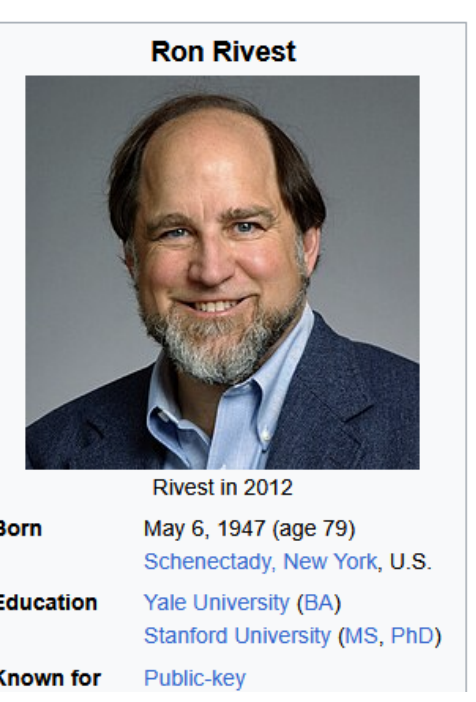
\includegraphics[width=52.08mm,height=193.05mm]{../../images/llm/page_041_img_01.png}%
\end{textblock*}

\end{document}
